\section{EXPERIMENT}
In this section, we first describe the testbed and then present the results of the experiments.

\subsection{Testbed}

\begin{figure}
  \centering
  \includegraphics[width=\columnwidth]{system-chart.png}
  \caption{Overall system configuration.}
  \label{fig:system}
\end{figure}

\begin{figure}
  \centering
  \begin{tabular}{cc}
      \begin{minipage}[t]{0.4 \columnwidth}
        \centering
        \includegraphics[keepaspectratio, scale=0.09]{chest.jpg}
        \subcaption{}
        \label{fig:chest}
      \end{minipage} &
      \begin{minipage}[t]{0.4 \columnwidth}
        \centering
        \includegraphics[keepaspectratio, scale=0.09]{chest_attach.jpg}
        \subcaption{}
        \label{fig:chest_attach}
      \end{minipage} \\
      \begin{minipage}[t]{0.4 \columnwidth}
        \centering
        \includegraphics[keepaspectratio, scale=0.09]{hand.jpg}
        \subcaption{}
        \label{fig:hand}
      \end{minipage} &
      \begin{minipage}[t]{0.4 \columnwidth}
        \centering
        \includegraphics[keepaspectratio, scale=0.051, angle=90]{hand_attach.jpg}
        \subcaption{}
        \label{fig:hand_attach}
      \end{minipage}
    \end{tabular}
  \caption{(a) Chest-mounted device, (c) wrist-mounted device for controlling the state of flapping drone. (b, d) the attachment of the devices.}
\end{figure}
\begin{figure}
  \centering
  \begin{tabular}{cc}
      \begin{minipage}[t]{0.4 \columnwidth}
        \centering
        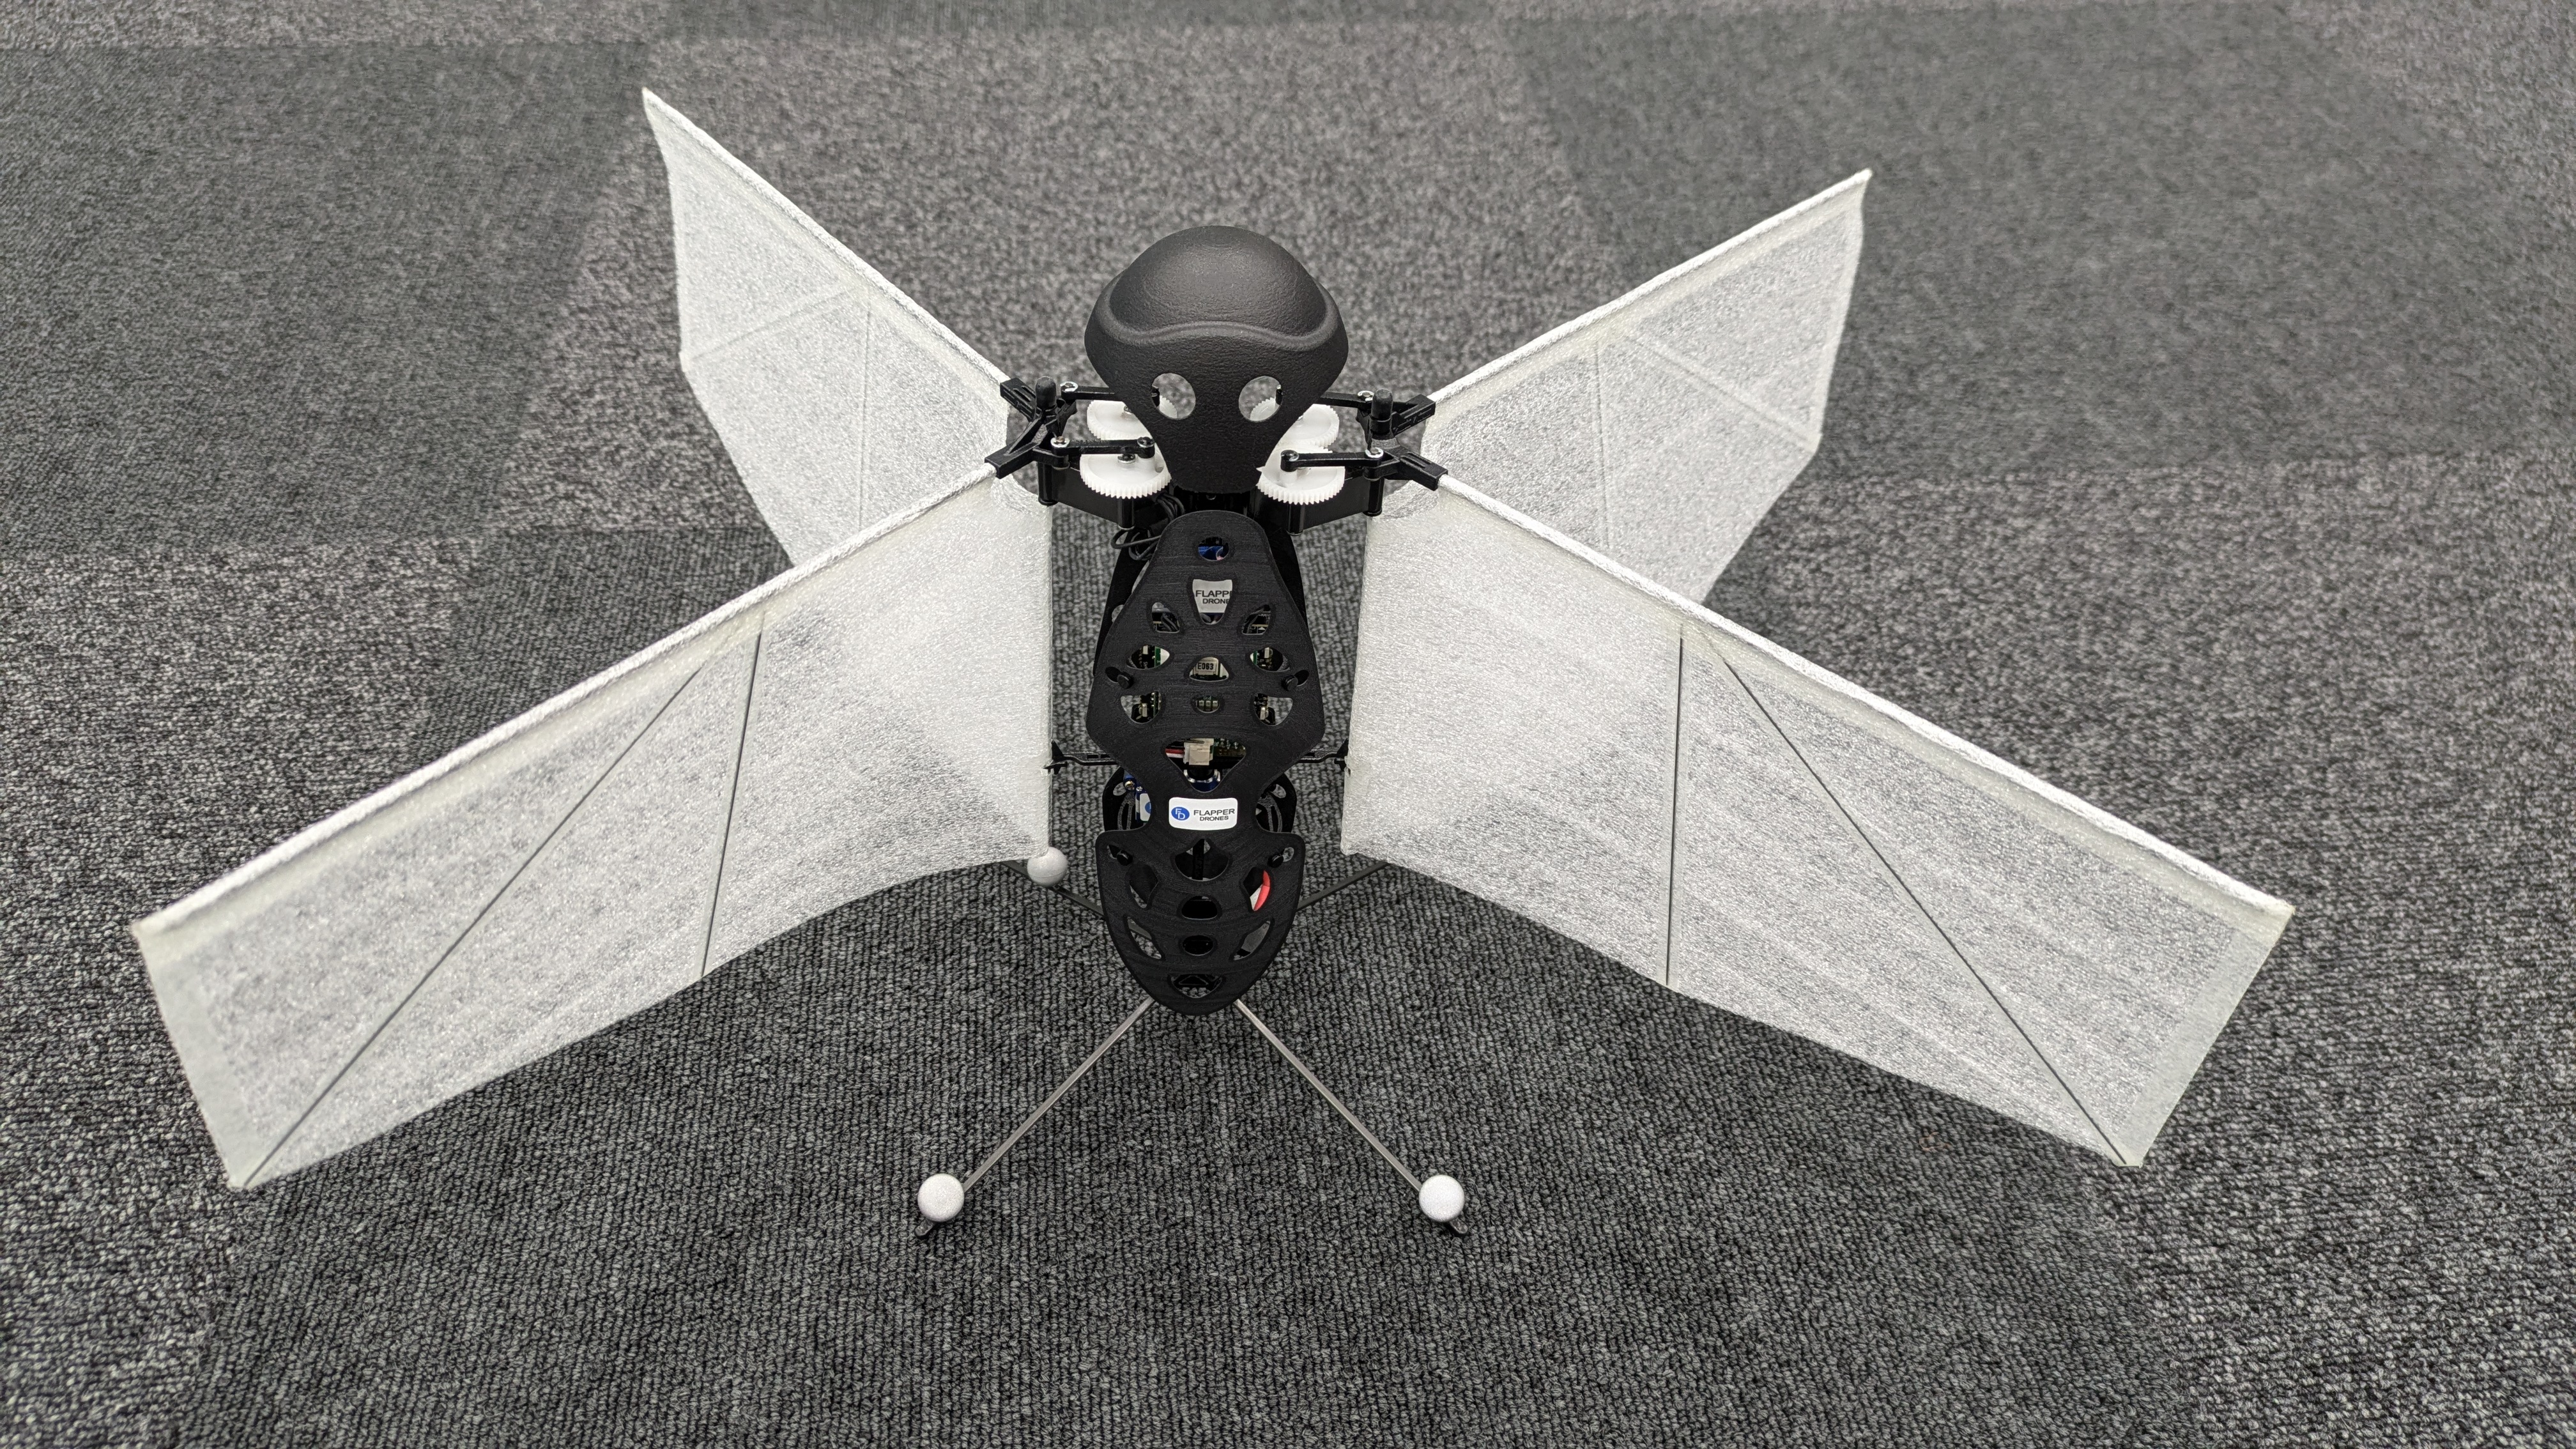
\includegraphics[keepaspectratio, scale=0.09]{flapper.jpg}
        \subcaption{}
        \label{fig:flapper}
      \end{minipage} &
      \begin{minipage}[t]{0.4 \columnwidth}
        \centering
        \includegraphics[keepaspectratio, scale=0.09]{leg.jpg}
        \subcaption{}
        \label{fig:leg}
      \end{minipage}
    \end{tabular}
  \caption{(a) Flapper Nimble+ drone, (b) its leg with motion capture markers.}
\end{figure}
Fig.~\ref{fig:system} illustrates the overall system configuration.
The system consists of a motion capture (MoCap) system, a flapping-wing drone, a user wearing devices, and a PC for trajectory planning and control.
The MoCap system tracks the 3D positions and orientations of the user's chest, palm, and the drone in real time.
We place 8 Optitrack Prime 13 cameras on the 4 corners and 4 sides of the room.  
The user wears chest-mounted and wrist-mounted markers allowing the system to capture intuitive control gestures. 
The PC processes the positional data and calculates the drone's optimal approach path toward the user's palm while maintaining a safe distance. 
The computed path is transmitted to the drone via a radio dongle, ensuring real-time control. 
The drone goes to the newest goal received from the PC using control in section~\ref{sec:modeling}, 
adjusting its motion dynamically based on feedback from the MoCap system.

Then, we describe the drone used in the experiment and the interface for control in detail.
Flapper Nimble+ used in the experiment, shown in Fig.~(\ref{fig:flapper}), is a flapping-wing drone by FLAPPER DRONES compatible with the Crazyflie software, 
which is a open-source platform for research and development of quadcopters produced by Bitcraze AB. 
As shown in Fig.~\ref{fig:leg} attached four motion capture markers on its legs for tracking its position and orientation. 
As noted in Section~\ref{sec:motion-planning}-\ref{fig:trajectory}, the drone has to change its behavior according to the position of the user's palm.
To facilitate intuitive control, we designed a wearable interface consisting of 
a chest-mounted device shown in Fig.~(\ref{fig:chest}) and 
a wrist-mounted device shown in Fig.~(\ref{fig:hand}).
Both devices were fabricated using a PLA 3D printer. 
With these devices, we acquire the user's palm position and orientation from the motion capture system and calculate the desired drone behavior based on the user's palm position. 
This interaction design only requires arm bending and streaching to switch the state of the drone and thus enables a seamless and intuitive approach control.
\subsection{Palm Landing Experiments}
\begin{figure}
    \begin{tabular}{cc}
      \centering
      \begin{minipage}[t]{0.45 \columnwidth}
        \centering
        \includegraphics[keepaspectratio, scale=0.09]{start.png}
        \subcaption{}
        \label{fig:start}
      \end{minipage}&
      \begin{minipage}[t]{0.45 \columnwidth}
        \centering
        \includegraphics[keepaspectratio, scale=0.09]{takeoff.png}
        \subcaption{}
        \label{fig:takeoff}
      \end{minipage} \\
      \begin{minipage}[t]{0.45 \columnwidth}
        \centering
        \includegraphics[keepaspectratio, scale=0.09]{approach.png}
        \subcaption{}
        \label{fig:approach}
      \end{minipage}&
      \begin{minipage}[t]{0.45 \columnwidth}
        \centering
        \includegraphics[keepaspectratio, scale=0.09]{palm-land.png}
        \subcaption{}
        \label{fig:palm-land}
      \end{minipage}      
    \end{tabular}
    \caption{The drone states during the experiment. (a) Start, (b) Takeoff, (c) Approach, (d) Palm landing.}
    \label{fig:states}
\end{figure}

\begin{figure}
        \begin{minipage}[t]{\columnwidth}
          \centering
          \includegraphics[keepaspectratio, scale=0.23]{simple-hand-landing-trajectory.png}
          \subcaption{}
          \label{fig:simple_hand_landing_trajectory}
        \end{minipage} \\
        \begin{minipage}[t]{\columnwidth}
          \centering
          \includegraphics[keepaspectratio, scale=0.29]{simple-hand-landing-vel.png}
          \subcaption{}
          \label{fig:simple_hand_landing_vel}
        \end{minipage} \\
        \begin{minipage}[t]{\columnwidth}
          \centering
          \includegraphics[keepaspectratio, scale=0.24]{XY_distances.png}
          \subcaption{}
          \label{fig:simple_hand_landing_xy_distances}
        \end{minipage}
    \caption{Results of the experiment. 
    (a) Trajectory and orientations of the drone during the approach.
    The red points indicates the actual positions of the drone during the approach and the blue points the target positions. 
    The arrows stemming from the red points indicate the orientation of the drone.
    The blue points start when the drone state becomes "APPROACH" as shown in Fig.~\ref{fig:simple_hand_landing_trajectory}.
    (b) Velocity profile of the drone during the approach. 
    The vertical dotted red line indicates the approach start time,
    the black line the time when the drone starts to decelerate,
    and the blue line the time when $k^\prime$ changes from 0.2 to 0.5.
    After the black line, the drone decelerates and the XY speed successfully decreases.
    (c) Distance between the user's chest and the drone during the approach.
}
\end{figure}

Fig.~\ref{fig:states} shows the drone states during the experiment.
We explain the results of the experiment in the following sections.

\subsubsection{Trajectory Mapping}
In Fig.~\ref{fig:trajectory}, it can be observed that the drone closely follows the planned trajectory and the drone's orientation always faces the user's chest.
To examine the precise time offset between the actual and target positions, we calculate the root mean square error (RMSE) between them based on different time offsets, which is shown in Table~\ref{tab:rmse}.
\begin{table}[t]
  \centering
  \caption{RMSE for Different Time Offsets}
  \begin{tabular}{cc}
      \toprule
      Time Offset (s) & RMSE (m) \\
      \midrule
      0.0 & 0.1695 \\
      0.1 & 0.1542 \\
      0.2 & 0.1391 \\
      0.3 & 0.1245 \\
      0.4 & 0.1092 \\
      0.5 & 0.0948 \\
      0.6 & 0.0813 \\
      0.7 & 0.0704 \\
      0.8 & 0.0620 \\
      0.9 & 0.0568 \\
      1.0 & 0.0554 \\
      1.1 & 0.0573 \\
      1.2 & 0.0635 \\
      1.3 & 0.0725 \\
      1.4 & 0.0840 \\
      1.5 & 0.0964 \\
      \bottomrule
  \end{tabular}
  \label{tab:rmse}
\end{table}
The table shows that the RMSE is minimized at a time offset of 1.0s, which indicates that the drone's actual position is approximately 1.0s behind the target position,
which is about ten times larger than the time interval $\Delta t$ of 0.1s.
This suggests that the drone's response time is significantly slower than expected from the Eq.~(\ref{eq:goal}).

\subsubsection{Velocity}
In Fig.~\ref{fig:simple_hand_landing_vel},
you can see that between the red and black lines, XY speed osscilates around a constant value, and between the black and blue lines, the XY speed decreases with oscillation.
The oscillation is considered to be due to the constantly updated goal position at a certain frequency.
From Eq.~(\ref{eq:weber}), the oscillation means the instability of $\Delta s$.,
which might cause a psychological threat to the user.
To mitigate this, we can consider increasing the frequency of the goal position update or using a smoother trajectory planning method.
Additionally, You can see a sudden increase right after the blue line, which is considered to be due to the acceleration caused by the change in $k^\prime$ as expected.

\subsubsection{Distance Between Chest and Drone}
As shown in Fig.~\ref{fig:simple_hand_landing_xy_distances}, the chest-drone distance and the drone-hand distance start decreasing 
when the chest-hand distance is above 0.3m.
The minimum distance between the drone and the user's chest is 0.693m.
The drone successfully keeps out of the chest-hand range.
Furthermore, the drone-hand distance gradually and smoothly decreases to zero without any overshoots,
which enables smoothe and safe palm-landing.